\section{Auswertung}

\subsection{Apparatekonstante}

Das Signal am Ausgang "Reference" ist regelbar, während das Signal am Ausgang "Oscillator" konstant bei
\SI{3,28}{\V} liegt.

\subsection{Messung des Ausgangssignals}

\subsubsection{ohne Noise \label{sec:knoise}}

Die Referenzspannung wurde auf $\SI{1}{\V}$ und $\SI{1000}{\Hz}$ eingestellt. Der Gain am Pre-Amplifier beträgt $10$.
In Abbildung \ref{fig:test} befinden sich die Spannungsverläufe der Ausgangsspannung bei unterschiedlichen Phasen.
\begin{figure}[H]
  \caption{Spannungsverläufe in Abhängigkeit von der Phase}
  \label{fig:test}
  \centering
        \begin{subfigure}[b]{0.48\textwidth}
                \centering
                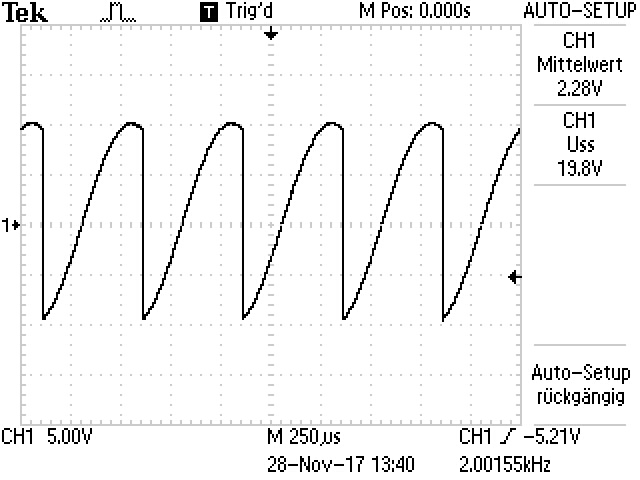
\includegraphics[width=\textwidth]{Text/Bilder/0.jpg}
                \caption{$\Phi = \SI{0}{°}$}
                \label{fig:gull}
        \end{subfigure}
        \quad
        \begin{subfigure}[b]{0.48\textwidth}
                \centering
                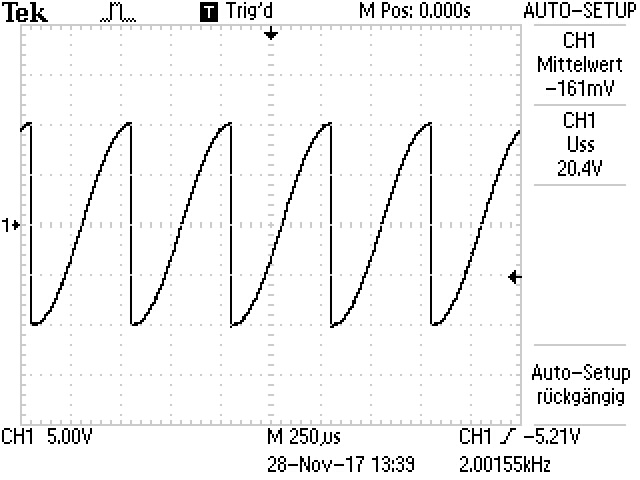
\includegraphics[width=\textwidth]{Text/Bilder/30.jpg}
                \caption{$\Phi = \SI{30}{°}$}
                \label{fig:gull2}
        \end{subfigure}
        \par\bigskip
        \begin{subfigure}[b]{0.48\textwidth}
                \centering
                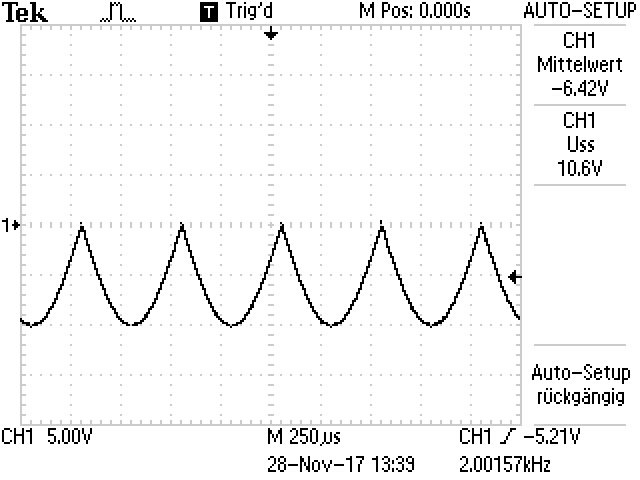
\includegraphics[width=\textwidth]{Text/Bilder/120.jpg}
                \caption{$\Phi = \SI{120}{°}$}
                \label{fig:gull3}
        \end{subfigure}
        \quad
        \begin{subfigure}[b]{0.48\textwidth}
                \centering
                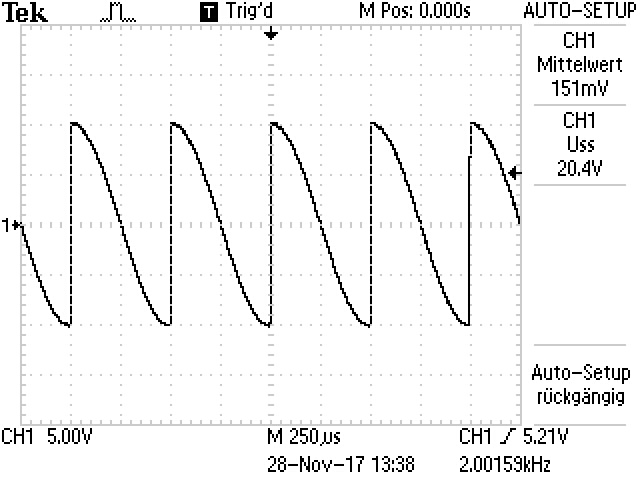
\includegraphics[width=\textwidth]{Text/Bilder/210.jpg}
                \caption{$\Phi = \SI{210}{°}$}
                \label{fig:gull4}
        \end{subfigure}
        \par\bigskip
        \begin{subfigure}[b]{0.48\textwidth}
                \centering
                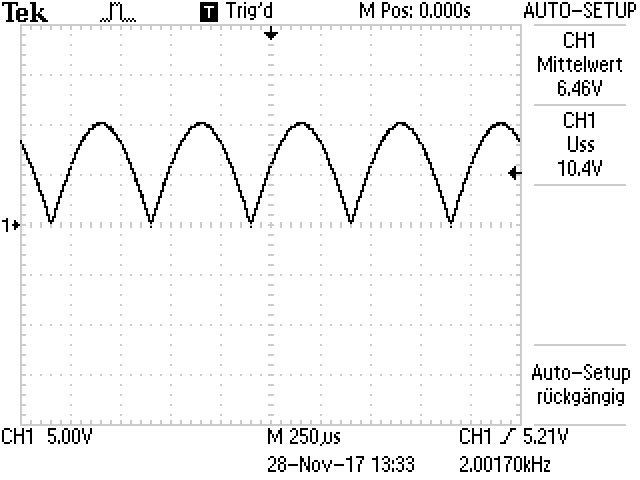
\includegraphics[width=\textwidth]{Text/Bilder/300.jpg}
                \caption{$\Phi = \SI{300}{°}$}
                \label{fig:gull5}
        \end{subfigure}
\end{figure}

\newpage
Die aufgenommenen Messwerte befinden sich in Tabelle \ref{tab:knoise}.
\begin{table}[H]
  \centering
  \caption{Messdaten "ohne Noise"}
  \label{tab:knoise}
  \begin{tabular}{c S}
    \toprule
      {$\Phi \:/\: \mathrm{°}$} & {$U_\text{out} \:/\: \mathrm{V}$}\\
    \midrule
    0  &	2,32        \\
    30	  &  -0,08 \\
    120  &  	-6,32 \\
    150  &  	-4,56 \\
    180  &  	-2,16 \\
    210  &  	0,32 \\
    240  &  	4,48 \\
    270  &  	6,00 \\
    300  &  	6,48 \\
    330  &  	4,88 \\
    \bottomrule
  \end{tabular}
\end{table}
%
%\newpage
%
Aus diesen Messwerten folgt der Graph:

\begin{figure}[H]
  \centering
  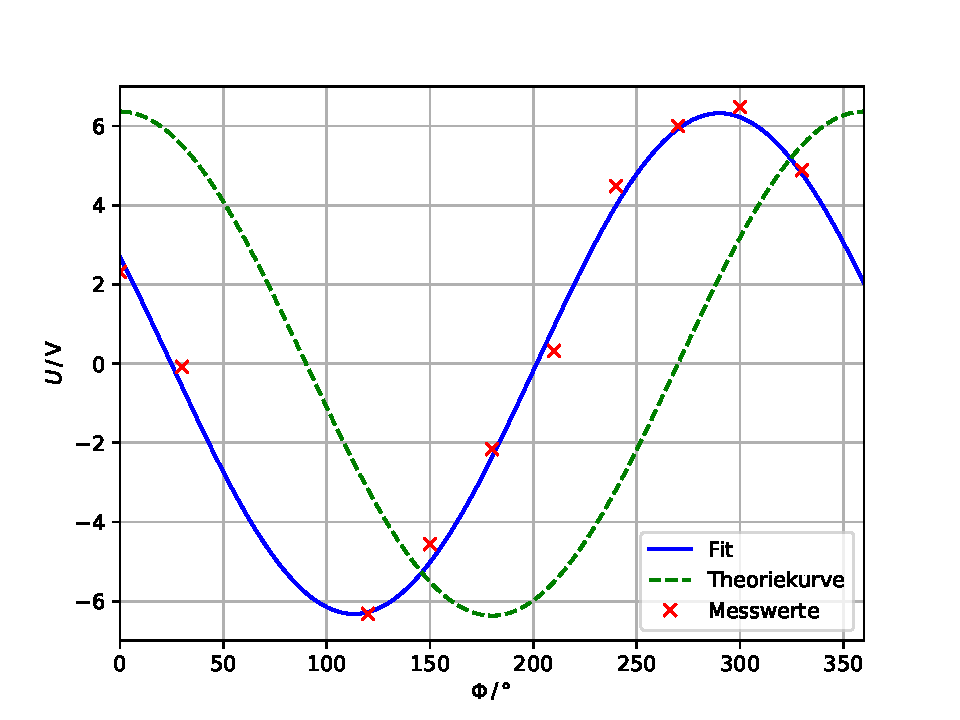
\includegraphics[width=\textwidth]{Plots/knoise.pdf}
  \caption{$U$-$\Phi$-Diagramm}
  \label{fig:knoise}
\end{figure}

Mithilfe der Messwerte wird die Regression $a \cdot \cos{(b \cdot x + c)}$ durchgeführt, die die Werte
\begin{align*}
  a &= \SI{6,32(21)}{\V} \\
  b &= 0,0178 \pm 0,0002 \\
  c &= \SI{64,78(304)}{°}
\end{align*}

liefert. Da die Theoriekurve aus Gleichung \eqref{eqn:Uout} die Werte
\begin{align*}
  a_\text{theo} &= \SI{6,37}{\V} \\
  b_\text{theo} &= 0,0175 \\
  c_\text{theo} &= \SI{0}{°}
\end{align*}

hat, ergeben sich die Abweichungen
\begin{align*}
  \delta_a &= 0,68 \% \\
  \delta_b &= 1,79 \%.
\end{align*}

% Die Fehler erhält man aus der Gauß'schen Fehlerfortpflanzung
% \begin{equation}
%    \delta = \sqrt{ \sum_{i=1}^{n}(\frac{\partial y}{\partial x_i} \Delta x_i)^2}.
%    \label{eqn:gaus}
%  \end{equation}


\subsubsection{mit Noise \label{sec:mnoise}}

Für diesen Teil des Experiments wurde der Noise auf $10^{-1}$ gestellt.
Die aufgenommenen Messwerte befinden sich in Tabelle \ref{tab:mnoise}.

\begin{table}[H]
  \centering
  \caption{Messdaten "mit Noise"}
  \label{tab:mnoise}
  \begin{tabular}{c S}
    \toprule
      {$\Phi \:/\: \mathrm{°}$} & {$U_\text{out} \:/\: \mathrm{V}$} \\
    \midrule
    0  & 	2,28      \\
    30	  & -0,40  \\
    120  & 	-6,24  \\
    150  & 	-4,40  \\
    180  & 	-2,16  \\
    210  & 	0,40  \\
    240  & 	4,48  \\
    270  & 	6,00  \\
    300  & 	6,40  \\
    330  & 	4,56  \\
    \bottomrule
  \end{tabular}
\end{table}

Aus diesen Messwerten folgt der Graph:

\begin{figure}[H]
  \centering
  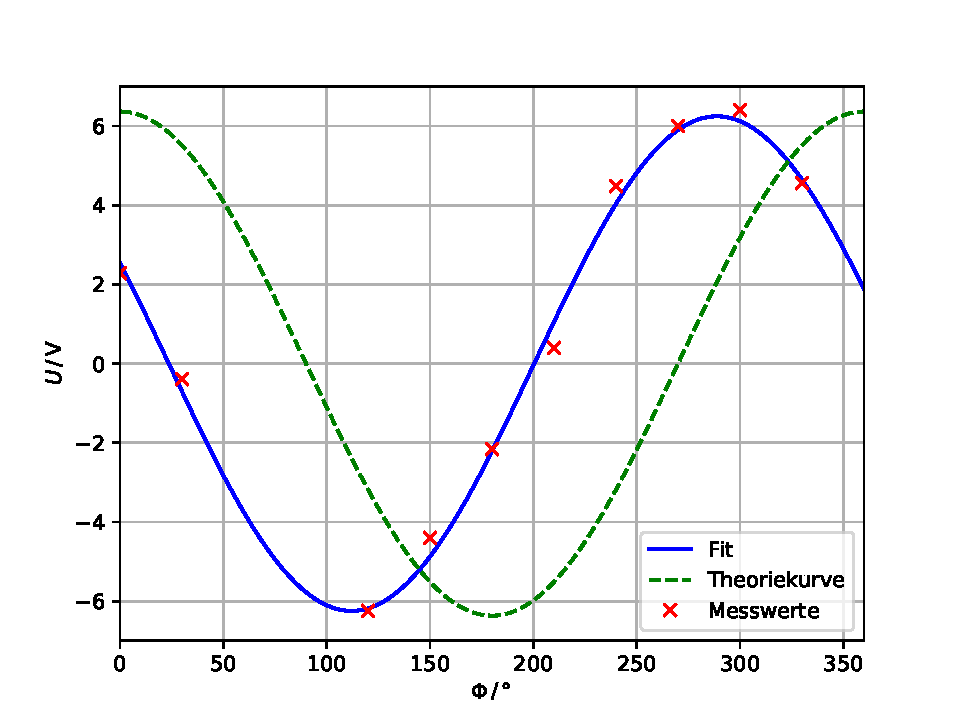
\includegraphics[width=\textwidth]{Plots/mnoise.pdf}
  \caption{$U$-$\Phi$-Diagramm}
  \label{fig:mnoise}
\end{figure}

Es wird erneut eine Regression durchgeführt. Sie liefert die Werte
\begin{align*}
  a &= \SI{6,25(19)}{\V} \\
  b &= 0,0178 \pm 0,0003 \\
  c &= \SI{65,97(279)}{°}.
\end{align*}

Die Theoriekurve ist dieselbe wie in \ref{sec:knoise}. Damit ergeben sich die Abweichungen
\begin{align*}
  \delta_a &= 1,90 \% \\
  \delta_b &= 1,80 \%
\end{align*}


\subsubsection{LED \label{sec:led}}
Die LED blinkt mit einer Frequenz von $\SI{300}{Hz}$ und der Gain am Pre-Amplifier beträgt $1000$.
Die aufgenommenen Messwerte befinden sich in Tabelle \ref{tab:led}.

\begin{table}[H]
  \centering
  \caption{Messdaten "LED"}
  \label{tab:led}
  \begin{tabular}{S S}
    \toprule
      {$r \:/\: \mathrm{cm}$} & {$U_\text{out} \:/\: \mathrm{V}$} \\
    \midrule
    2,8  & 	-2,00    \\
    3,8	  &  -1,44  \\
    4,8	  &  -0,88  \\
    5,8	  &  -0,56  \\
    6,8	  &  -0,40  \\
    7,8	  &  -0,32  \\
    8,8	  &  -0,24  \\
    9,8	  &  -0,16  \\
    10,8  &  	-0,08  \\
    11,8  &  	-0,08  \\
    12,8  &  	0,00  \\
    \bottomrule
  \end{tabular}
\end{table}

Zur Erstellung der Grafik wurden die Beträge der gemessenen Spannungen gegen die Abstände aufgetragen.

\begin{figure}[H]
  \centering
  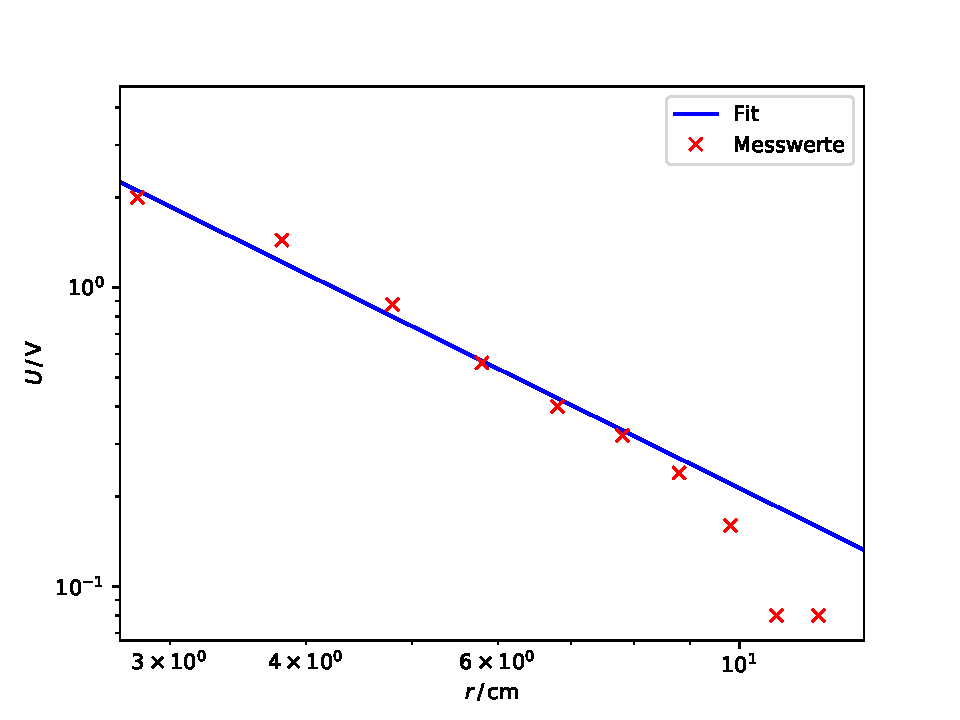
\includegraphics[width=\textwidth]{Plots/led.pdf}
  \caption{$U$-$r$-Diagramm zur Bestimmung der Steigung}
  \label{fig:led}
\end{figure}

Dieses mal ergibt die Regression $a \cdot x^{-b}$ die Steigung
\begin{equation*}
  b = 1,80 \pm 0,13
\end{equation*}

Da die Intensität mit $\sfrac{1}{r^2}$ abfällt ist der Theoriewert
\begin{equation*}
  b_\text{theo} = 2.
\end{equation*}

Die Abweichung beträgt somit
\begin{equation*}
  \delta = 9,88 \%.
\end{equation*}

Der maximale Abstand, bei dem das Licht der LED noch nachgewiesen werden konnte, beträgt
\begin{equation*}
  r_\text{max} = \SI{11,8}{\cm}.
\end{equation*}
